\chapter{Результат}

На рисунке \ref{fig:gui} представлен графический интерфейс приложения.

\begin{figure}[H]
	\centering
	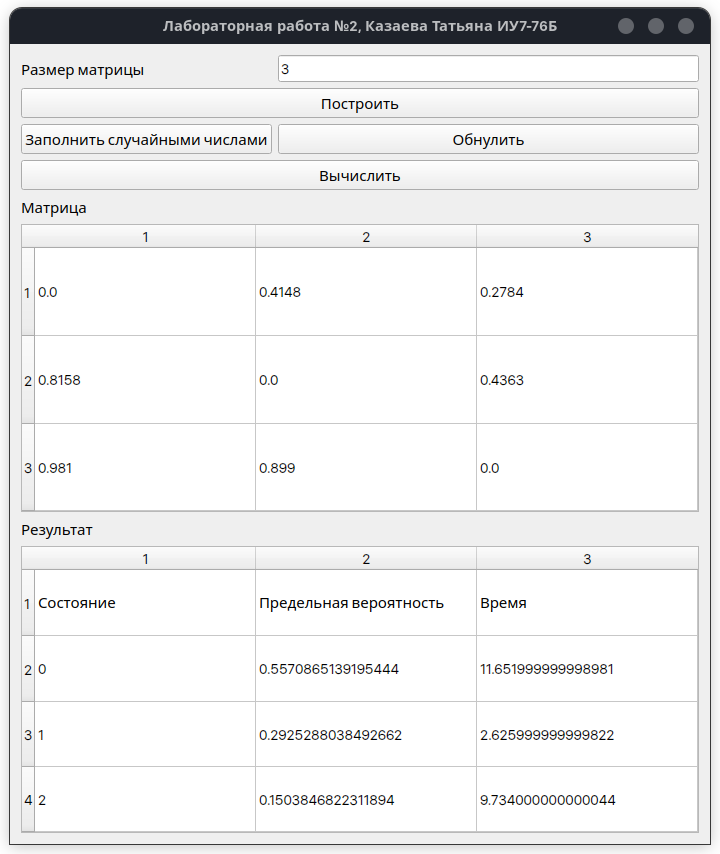
\includegraphics[width=0.8\linewidth]{assets/gui.png}
	\caption{Графический интерфейс приложения}
	\label{fig:gui}
\end{figure}

Пользователь может как редактировать матрицу вручную, так и заполнить её случайными числами,
нажав на соответствующую кнопку. Также пользователь может заполнить таблицу нулями, нажав на кнопку <<занулить>>.